\documentclass[11pt]{beamer}
\usepackage{helvet} %font
\beamertemplatenavigationsymbolsempty
\usetheme{JuanLesPins}
\usefonttheme{structurebold}

\usepackage[french]{babel}
\usepackage[utf8]{inputenc}
\usepackage[T1]{fontenc}
\usepackage{amssymb,amsmath}
\usepackage{tikz}
\usepackage{geometry}
\usepackage{xcolor,colortbl}
\usetikzlibrary{arrows,positioning}
\usepackage{listings}

\AtBeginSubsection[]
{
   \begin{frame}
	\small \tableofcontents[currentsection]
   \end{frame}
}

\newenvironment{slide}[1]{%
\begin{frame}[environment=slide]
\frametitle{#1}
}{%
\end{frame}
}
\setbeamercolor{structure}{fg=red}
\setbeamercolor{frametitle}{bg=black,fg=white}
\definecolor{gris}{gray}{0.6}
\definecolor{grisclair}{gray}{0.9}

\newtheorem{exercice}{Exercice}

\title{Machine Learning VI \\ Méthodes avancées}
\author{Nicolas Bourgeois}
\date{}

\newcommand{\Python}[1]{
	{\small	\lstinputlisting[language=Python]{./#1.py}}
}
\newenvironment{pyenvsmall}
	{ \ttfamily \tiny }
	{\par  }

\newcommand{\Pythonsmall}[1]{
	{\scriptsize \lstinputlisting[language=Python]{./#1.py}}
}
\newcommand{\elimine}[1]{{\textcolor{lightgray}{#1}}}

\newcommand\Wider[2][3em]{%
\makebox[\linewidth][c]{%
  \begin{minipage}{\dimexpr\textwidth+#1\relax}
  \raggedright#2
  \end{minipage}%
  }%
}

\begin{document}

\begin{frame}
\maketitle
\end{frame}


\begin{frame}
\begin{columns}

\begin{column}{0.15\linewidth}
\centering
\begin{figure}

\includegraphics[width=0.8\textwidth]{./topics.png}
\end{figure}
\end{column}

\begin{column}{0.65\linewidth}
\centering
\begin{figure}
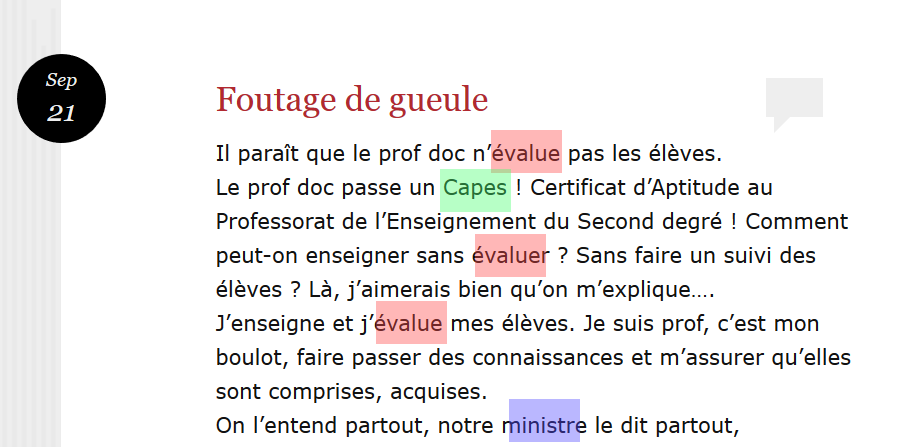
\includegraphics[width=\textwidth]{./blogaladoc2.png}
\end{figure}
\end{column}

\end{columns}

\vspace{0.3cm}

\begin{itemize}
\item chaque \textbf{topic} est une distribution de mots
\pause
\item chaque \textbf{document} est un mélange de quelques topics
\pause
\item chaque \textbf{mot} est tiré au sort dans un topic
\end{itemize}
\end{frame}

\begin{frame}
\begin{columns}

\begin{column}{0.15\linewidth}
\centering
\begin{figure}

\includegraphics[width=0.7\textwidth]{./topics_inconnus.png}
\end{figure}
\end{column}

\begin{column}{0.65\linewidth}
\centering
\begin{figure}
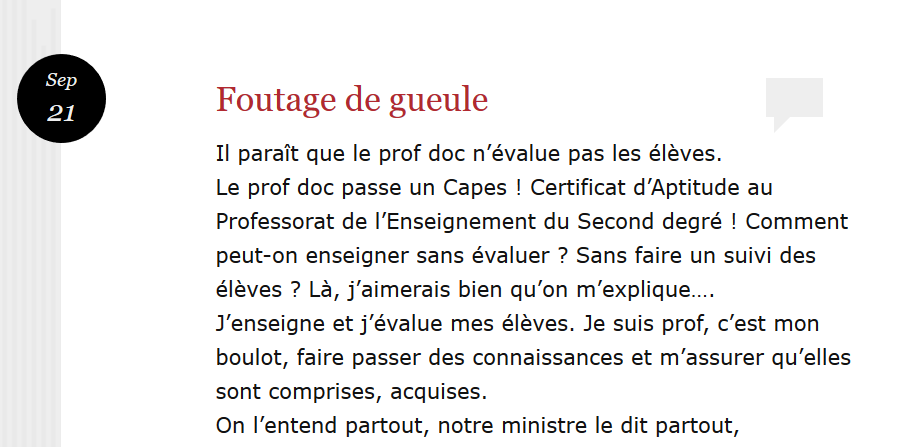
\includegraphics[width=\textwidth]{./blogaladoc.png}
\end{figure}
\end{column}

\end{columns}

\begin{itemize}
\item Dans la réalité, on observe les documents
\pause
\item Tout le reste constitue des \textbf{variables cachées}
\item Nous cherchons à les retrouver, en inversant le processus génératif
\end{itemize}
\end{frame}

\begin{frame}

\vspace{1.5cm}

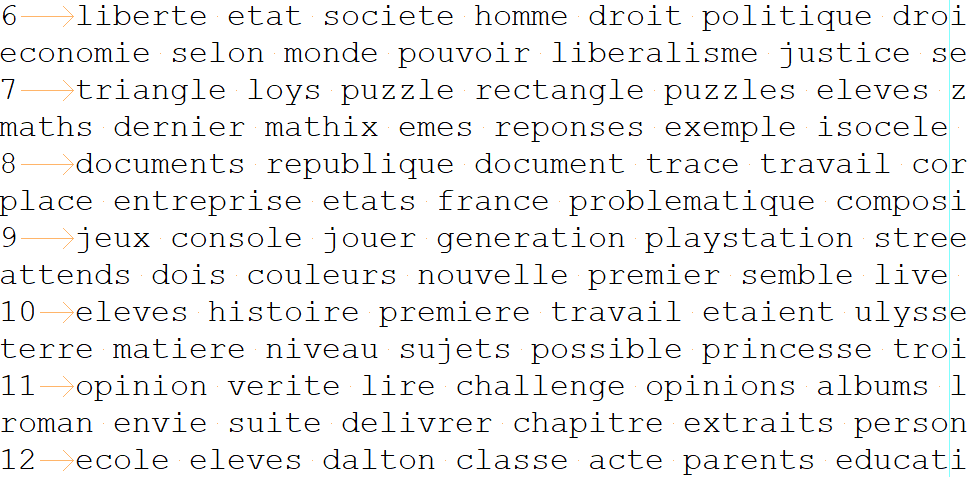
\includegraphics[scale=0.2]{code4-clefs.png}

\end{frame}

\begin{frame}
\vspace{1.5cm}

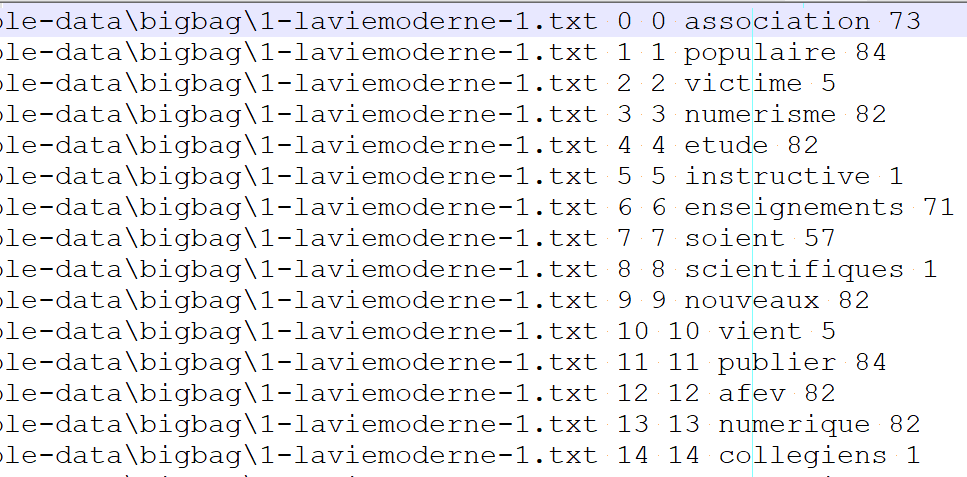
\includegraphics[scale=0.25]{code4-mots.png}

\end{frame}


\begin{frame}{Exercice}

\begin{exercice}
Entraînez un topic model sur les éléments 500 à 1000 du dataset \texttt{fetch\_20newsgroups}, pour une valeur de 10 topics. Affichez les 20 clefs principales des modèles fournis par le modèle.
\end{exercice}

\begin{exercice}
Codez une fonction de prétraitement pour enlever les scories, puis ré-entraînez le modèle et évaluez l'amélioration. Quelles autres pistes d'améliorations devraient être explorées ?
\end{exercice}

\end{frame}

\begin{frame}{Résultat attendu (1)}
Topic 0: does god evidence don reason know think like use believe\\

Topic 1: point right think people way just don law islam does\\

Topic 2: cubs think suck good players time really numbers world league\\

Topic 3: people said god say don just know like says did\\

Topic 4: ax max a86 b8f pl 1t qq bhj qax bj\\

Topic 5: like know use ve does want just good data bus\\

Topic 6: game space shuttle play period blues ny power 12 14\\

Topic 7: key keys encryption 20 chips 16 chip 15 10 use\\

Topic 8: windows file nt sec ram swap use dos da disk\\

Topic 9: db mov bh si cs byte al bl di maxbyte\\

Topic 0: does god evidence don reason know think like use believe

\end{frame}

\begin{frame}{Résultat attendu (2)}
\vspace{-0.1cm}Topic 0: windows know does believe think question people human good used\\

Topic 1: government shuttle nasa space just encryption people attitude font satellite\\

Topic 2: bits byte push picture loop offset east data west stuff\\

Topic 3: evidence local like read people keys physical transfer company rate\\

Topic 4: like really problem drives rotor problems hear lopez usual year\\

Topic 5: cubs suck just like rights year people think printer\\

Topic 6: just know good swap blues does think need drive power\\

Topic 7: pick koresh like batf just thanks think know right space\\

Topic 8: like people does just know said went going think good\\

Topic 9: israel just want people islam israeli time little lebanese peace\\

\end{frame}

\begin{frame}{Solution (1)}
\Pythonsmall{ex601}
\end{frame}

\begin{frame}{Solution (2)}
\Pythonsmall{ex602}
\end{frame}


\begin{slide}{}
	Qu'est-ce que c'est ?\\ \vspace{0.2cm}
	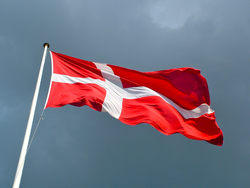
\includegraphics[scale=1]{danish_flag.png}
\end{slide}

\begin{slide}{}
	Quelle est son origine ?\\ \vspace{0.2cm}
	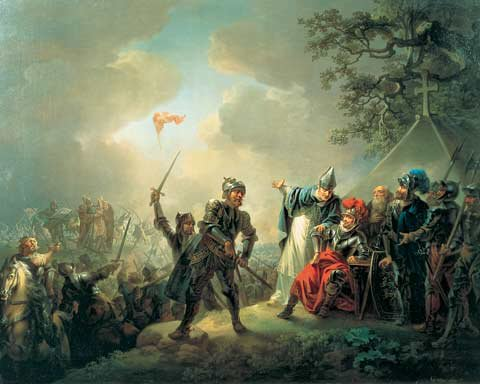
\includegraphics[scale=2.5]{Anders_Sunesen.jpg}
\end{slide}

\begin{slide}{La Livonie, XII\up{e}-XIII\up{e} siècles}
\begin{center}
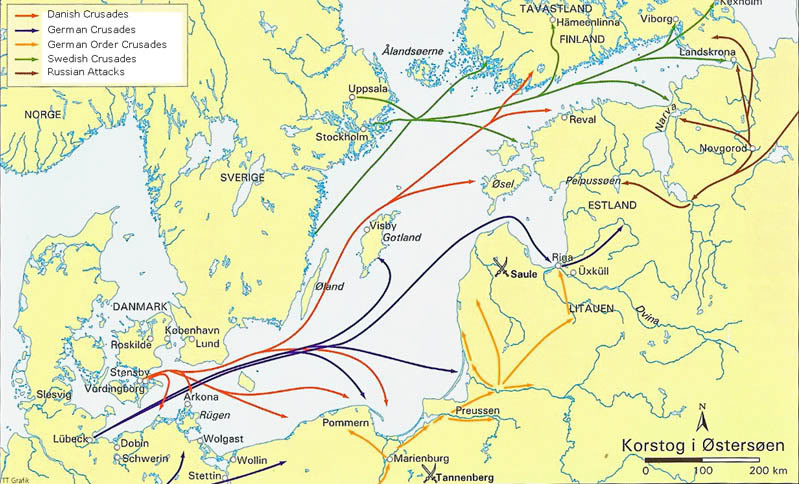
\includegraphics[scale=0.37]{crusades.jpg}
\end{center}
\end{slide}

\begin{slide}{Le texte d'Henri}
\begin{center}
\begin{tabular}{cc}
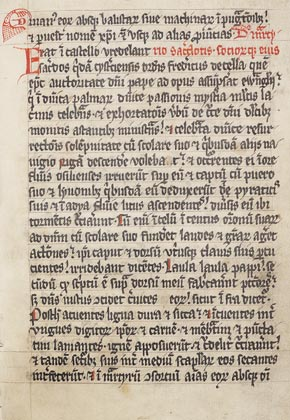
\includegraphics[scale=0.4]{HL.jpg} &
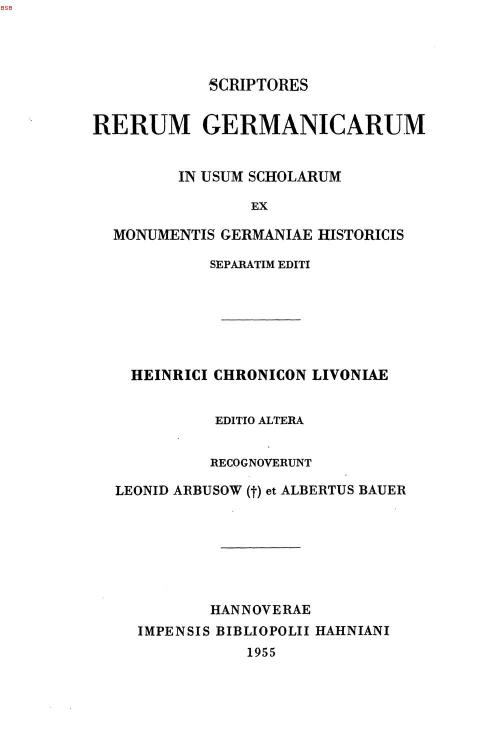
\includegraphics[scale=0.3]{MGH.jpeg}
\end{tabular}
\end{center}
\end{slide}

\begin{slide}{Carte de Kohonen}
\begin{center}
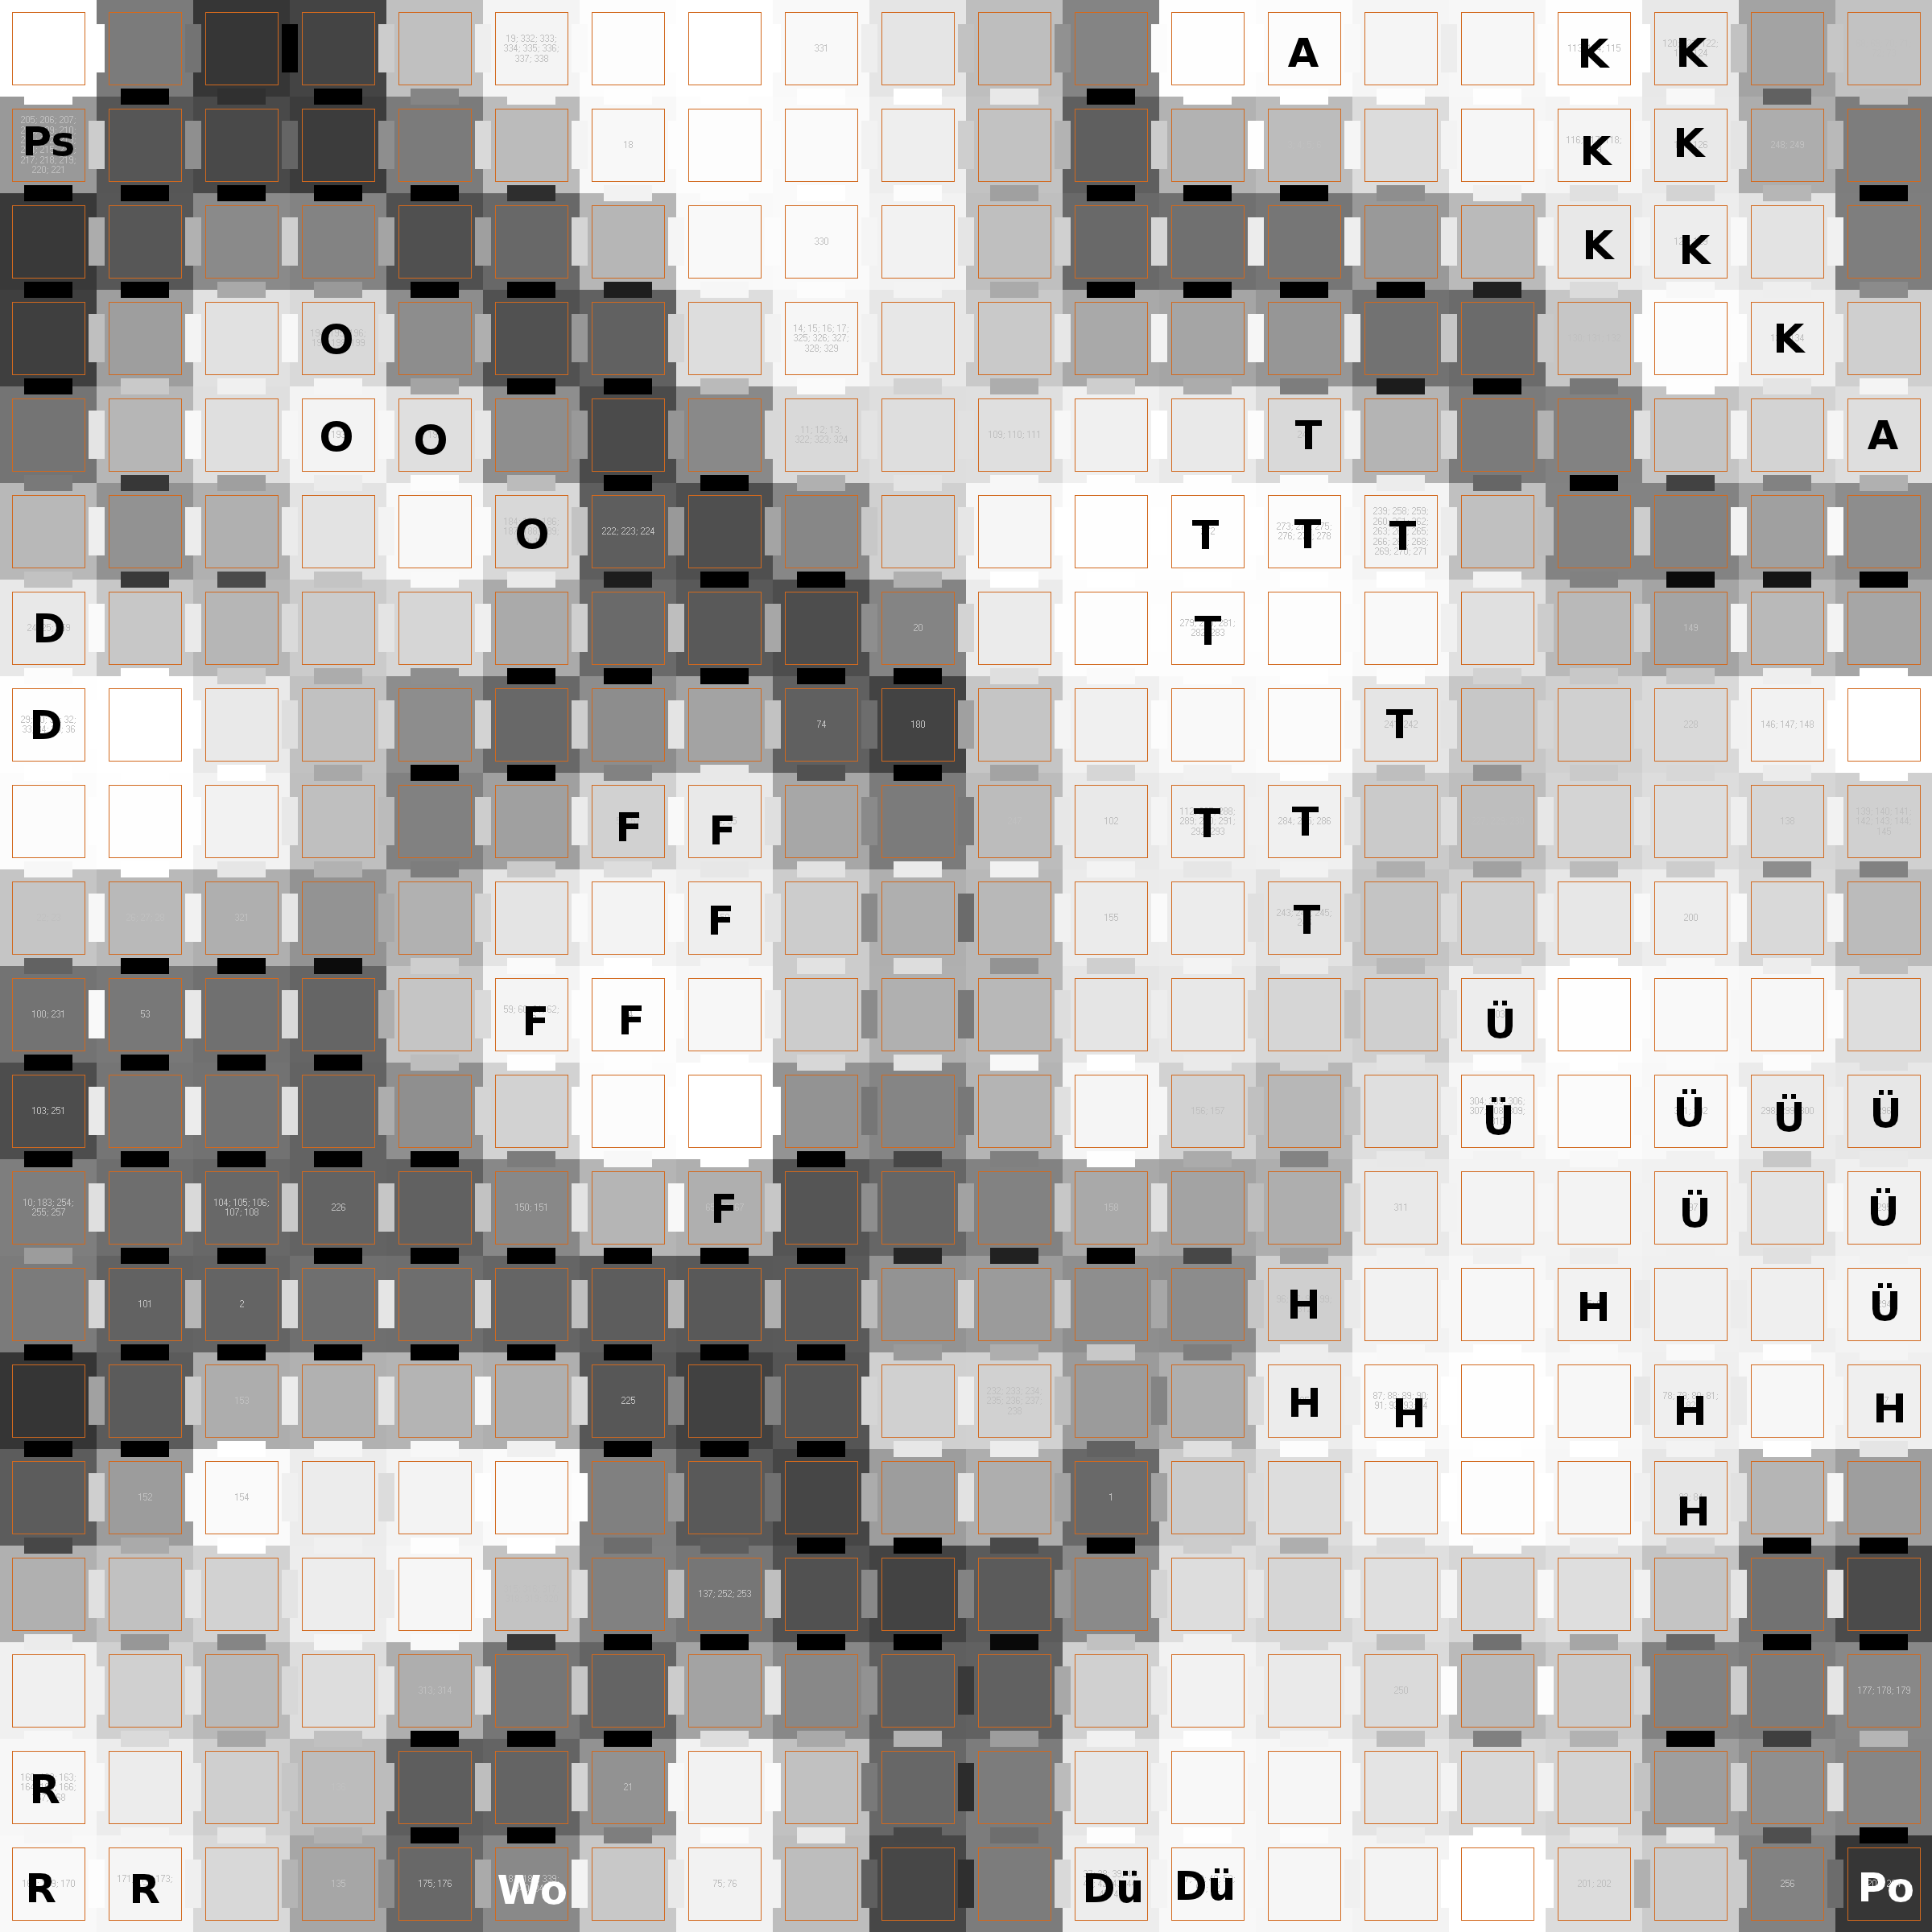
\includegraphics[scale=0.07]{HL_Kohonen.png}
\end{center}
\end{slide}


\begin{slide}{Kohonen Map}
\begin{center}
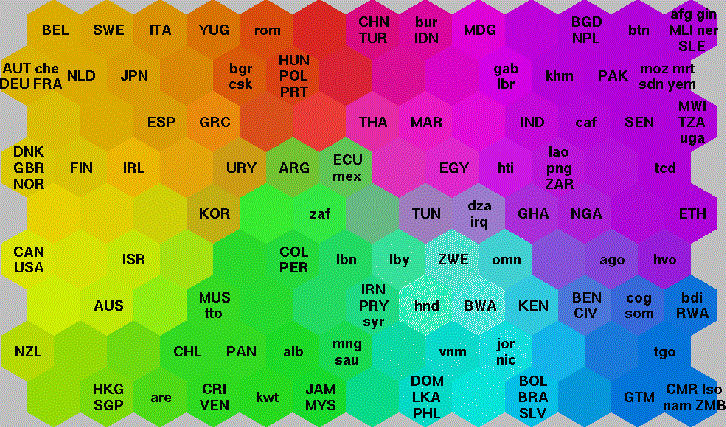
\includegraphics[scale=0.35]{povertymap}
\end{center}
\end{slide}

\begin{slide}{Kohonen Map}
\Pythonsmall{som1-extract}
\end{slide}

\begin{slide}{Kohonen Map}
\begin{center}
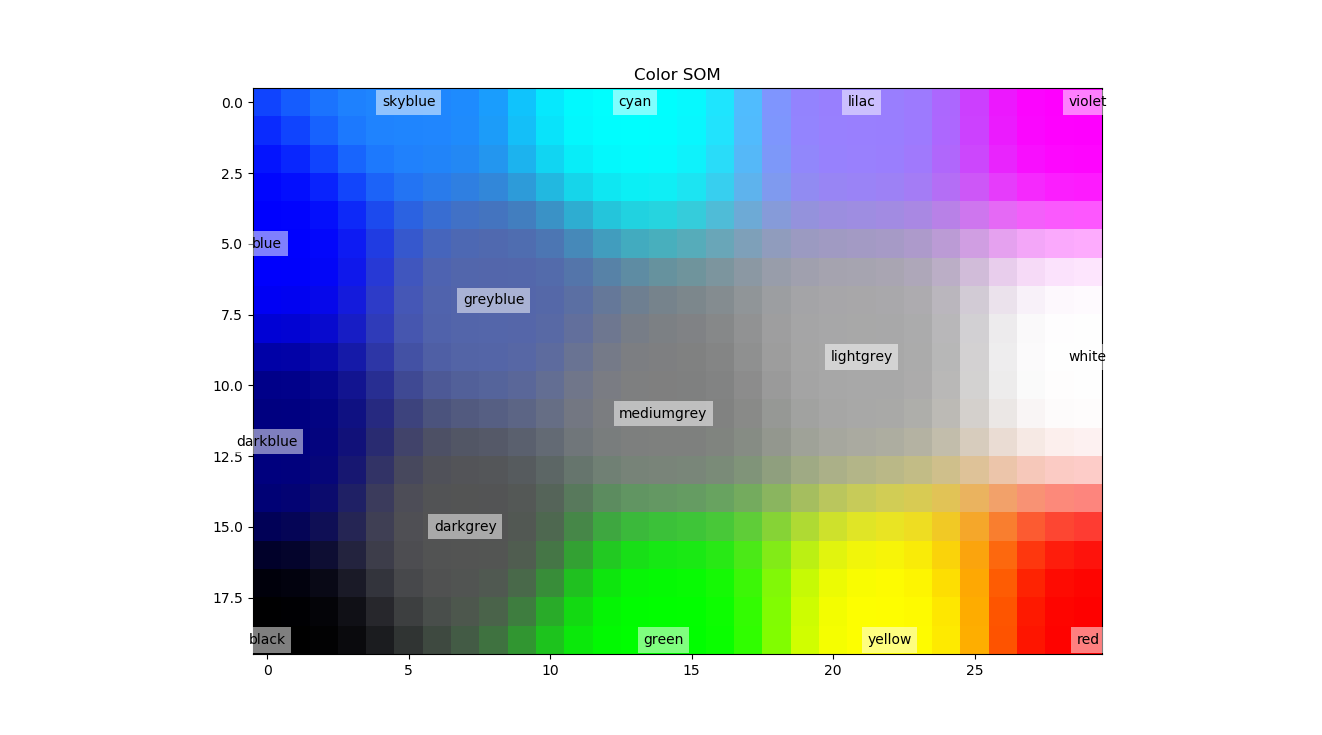
\includegraphics[scale=0.35]{som_exemple1}
\end{center}
\end{slide}


\begin{frame}{Exercice}

\begin{exercice}
Installez tensorfow et placez \texttt{C4/som1.py} dans le répertoire courant. Entraînez une carte auto-organisatrice sur \texttt{C4/data1.csv} avec une grille carrée $10 \times 10$. Affichez le résultat.
\end{exercice}
\end{frame}

\begin{frame}{Résultat attendu}
\begin{center}
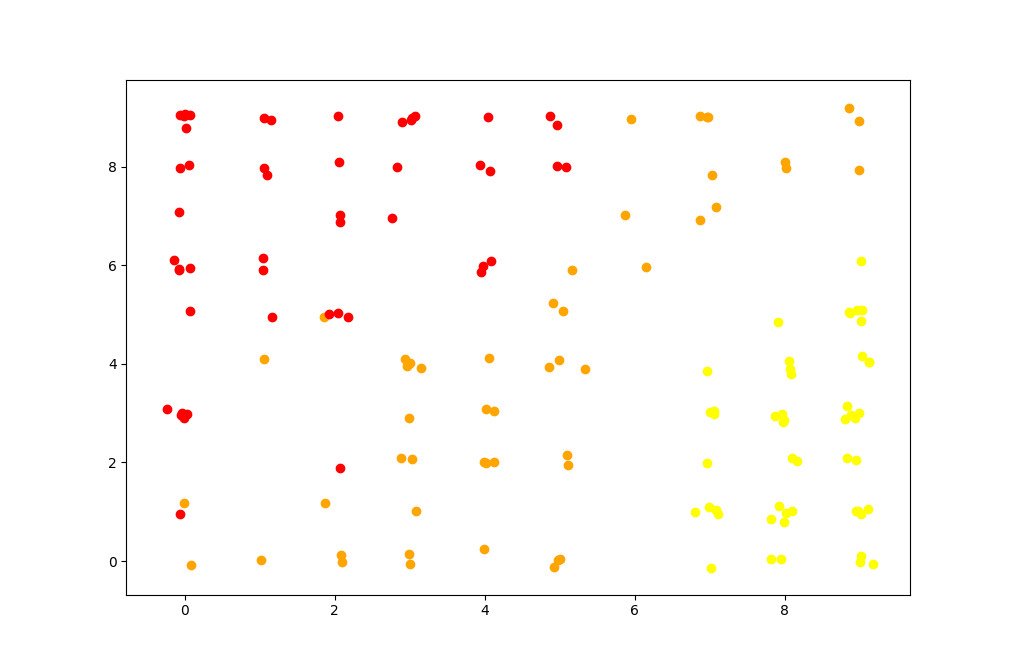
\includegraphics[scale=0.4]{ex603}
\end{center}
\end{frame}

\begin{frame}{Solution}
\Pythonsmall{ex603}
\end{frame}



\begin{frame}{Exercice}

\begin{exercice}
Produisez un schéma de test semblable à celui que je vous ai montré à la séance 4 à partir des générateurs de la librairie datasets (et de matplotlib bien sûr). 
\end{exercice}
\end{frame}

\begin{frame}{Résultat attendu}
\begin{center}
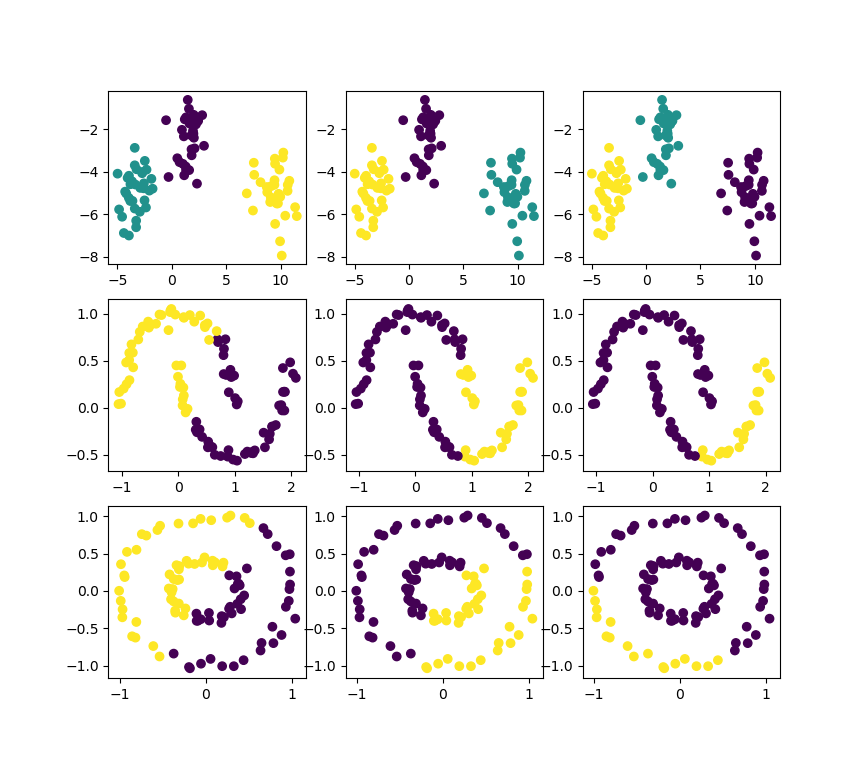
\includegraphics[scale=0.4]{ex700}
\end{center}
\end{frame}

\end{document}